% FONTE TEMA https://github.com/matze/mtheme
\documentclass[aspectratio=1610]{beamer}
%\documentclass[aspectratio=1610, handout]{beamer}
\usepackage[utf8]{inputenc}
\usepackage{ragged2e}
\usepackage{xcolor}
\usepackage[italian]{babel}
\usepackage{multirow}
\usepackage{silence}
\WarningFilter{beamer}{}
\WarningFilter{metropolis}{}
\usetheme[progressbar=frametitle,titleformat=smallcaps]{metropolis}
\setbeamertemplate{frame numbering}[fraction]
\setbeamercovered{dynamic}
\definecolor{rosso}{RGB}{255, 0, 0}
\definecolor{giallo}{RGB}{254,212,23}
\hypersetup{colorlinks=true,linkcolor=black,urlcolor=rosso}
\setbeamercolor{palette primary}{fg=black, bg=giallo}
\setbeamercolor{background canvas}{bg=white}
\setbeamercolor{normal text}{fg=black}
\setbeamercolor{progress bar}{fg=rosso}
\setbeamercolor{framesubtitle}{fg=rosso}
\setbeamercolor{normal text .dimmed}{fg=giallo}
\setbeamercolor{block title alerted}{fg=rosso, bg=giallo}
\setbeamerfont{caption}{size=\tiny}
\setbeamerfont{caption name}{size=\tiny}
\setlength{\abovecaptionskip}{0pt}
\makeatletter
\metroset{block=fill}
\setlength{\metropolis@progressinheadfoot@linewidth}{1pt} 
\setlength{\metropolis@progressonsectionpage@linewidth}{1pt}
\setlength{\metropolis@titleseparator@linewidth}{1pt}
\makeatother

\title{SOCIAL NETWORK E PROFILAZIONE}
\subtitle{Il modello di business dei social network}
\date{}
\institute{\textit{
        Fonti:
        \begin{itemize}
            \item[-] \href{https://it.wikipedia.org/wiki/Dark_pattern}{Wikipedia: dark pattern}
            \item[-] \href{https://www.enbilab.com/it/blog/pubblicita-comportamentale-o-contestuale-ecco-le-differenze}{Enbilab: pubblicità comportamentale vs contestuale}
            \item[-] \href{https://www.wired.it/attualita/tech/2020/09/24/social-dilemma-dopamina-effetto-smartphone-cervello}{Wired: come uno smartphone hackera il nostro cervello}
            \item[-] \href{https://guerredirete.substack.com/p/guerre-di-rete-dove-e-finita-letichetta}{Guerre di Rete: dove è finita l'etichetta AI}
        \end{itemize}
    }
}

\begin{document}

\begin{frame}[plain, noframenumbering]
    \titlepage
\end{frame}

\section{IL MODELLO DI BUSINESS DEI SOCIAL NETWORK}

\begin{frame}{IL MODELLO DI BUSINESS DEI SOCIAL NETWORK}
    \begin{alertblock}{I SOCIAL NETWORK SONO GRATUITI?}
        \begin{minipage}{0.98\linewidth}
            \justifying
            \begin{enumerate}
                \pause
                \item \textbf{SOLDI}: obiettivo primario dei social network è fare soldi;
                \pause
                \item \textbf{PUBBLICIT\'A}: la pubblicità è il mezzo principale per fare soldi;
                \pause
                \item \textbf{TEMPO}: per vendere pubblicità, i social network devono catturare la nostra attenzione il più a lungo possibile;
                \pause
                \item \textbf{DATI}: per catturare la nostra attenzione, i social network devono conoscere i nostri gusti, le nostre preferenze, le nostre abitudini, ecc... e per fare questo ci profilano continuamente.
            \end{enumerate}
            \bigskip
            \tiny{\textbf{Documentario}}\\
            \tiny{\href{https://thesocialdilemma.com/}{The Social Dilemma}}
        \end{minipage}
    \end{alertblock}
\end{frame}

\begin{frame}{QUANTI SOLDI?! ESEMPIO: FATTURATO TIK TOK}
    \begin{figure}
        \href{https://www.businessofapps.com/data/tik-tok-statistics/}{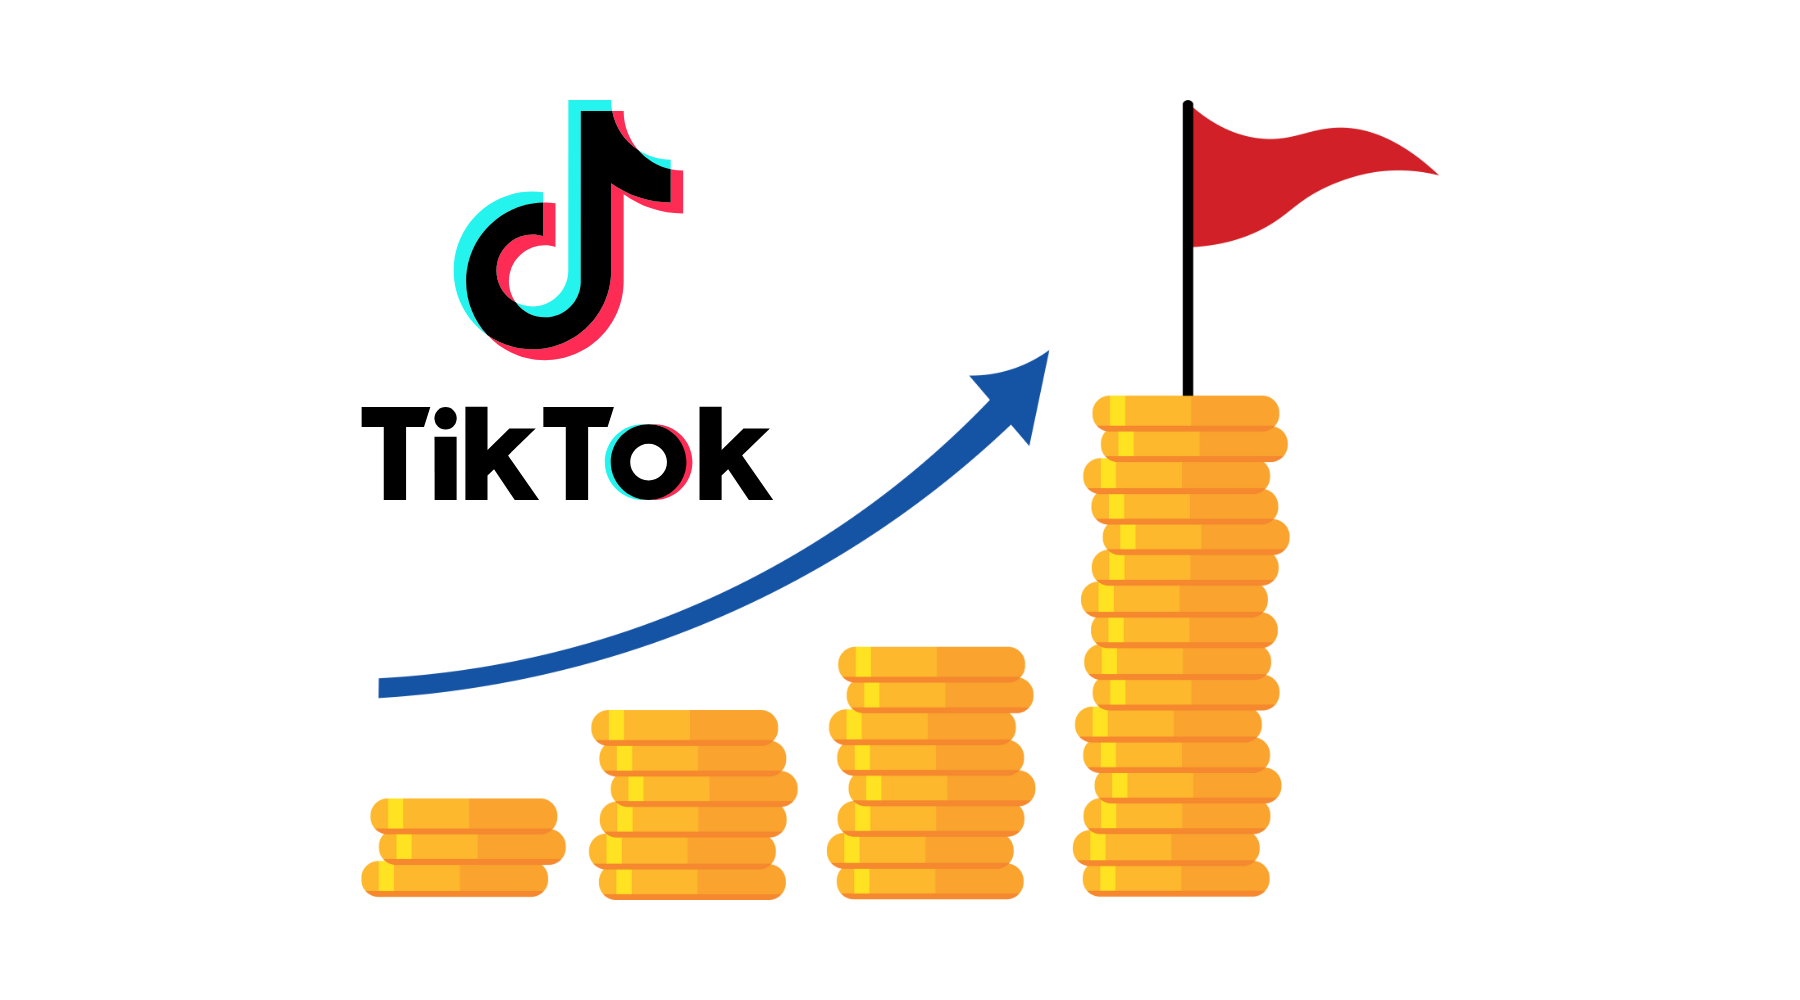
\includegraphics[width=\linewidth]{img/tiktok_1.png}}
        \caption{{creata con \href{https://www.canva.com}{Canva}}}
    \end{figure}
\end{frame}

\begin{frame}{PUBBLICIT\'A COMPORTAMENTALE VS CONTESTUALE}
    \begin{columns}
        \column{.5\textwidth}
            \begin{alertblock}{COMPORTAMENTALE}
                \begin{minipage}{0.96\linewidth}
                    \justifying
                    La pubblicità comportamentale, nota come ``Online Behavioral Advertising'' (\textbf{OBA}), 
                    si basa sulla raccolta di dati, anche tramite cookie, dell’attività online di 
                    un utente e del suo comportamento online, al fine di fornirgli annunci su misura, 
                    basati sui suoi interessi.\\
                    \bigskip
                    \tiny{\textbf{Approfondimento}}\\
                    \tiny{\href{https://attivissimo.me/2024/09/06/podcast-rsi-gli-smartphone-ci-ascoltano-no-ma}{Gli smartphone ci ascoltano?}}
                \end{minipage}
            \end{alertblock}
        \column{.5\textwidth}
            \begin{alertblock}{CONTESTUALE}
                \begin{minipage}{0.96\linewidth}
                    \justifying
                    La pubblicità contestuale (\textbf{contextual advertising}) si basa invece sul contenuto 
                    del sito in cui compare l’annuncio e non sui dati di navigazione. Gli annunci sono 
                    quindi pertinenti al contenuto della pagina web che l’utente sta visitando in quel 
                    momento.\\ 
                    \bigskip
                    \tiny{\textbf{Approfondimento}}\\
                    \tiny{\href{https://www.geopop.it/come-funzionano-le-pubblicita-personalizzate-online-il-ruolo-dei-cookie-e-la-nostra-privacy/}{Perchè rifiutare i cookie?}}
                \end{minipage}
            \end{alertblock}
    \end{columns}
\end{frame}

\begin{frame}{CATTURARE L'ATTENZIONE E CREARE DIPENDENZA}
    \begin{columns}
        \column{.6\textwidth}
            \begin{alertblock}{DIPENDENZA DAI SOCIAL NETWORK}
                \begin{minipage}{0.96\linewidth}
                    \justifying
                    \textbf{Ogni singola volta} che otteniamo un like, un commento o una qualunque notifica 
                    tutti noi riceviamo una piccola gratificazione, che a livello fisico è in realtà 
                    una scarica di \textbf{dopamina} e che sta alla base della nostra \textbf{dipendenza dai social 
                    network} (e, più in generale, degli \textbf{smartphone}).\\
                    Il meccanismo che regola tutto ciò è mutuato dal gioco d’azzardo e 
                    dalle slot machine ed è chiamato \textbf{sistema di rinforzo intermittente positivo}.\\
                    \bigskip
                    \tiny{\textbf{Fonte}}\\
                    \tiny{\href{https://www.wired.it/attualita/tech/2020/09/24/social-dilemma-dopamina-effetto-smartphone-cervello}{Dopamina e ricompense: come uno smartphone hackera il nostro cervello}}
                \end{minipage}
            \end{alertblock}
        \column{.4\textwidth}
            \begin{figure}
                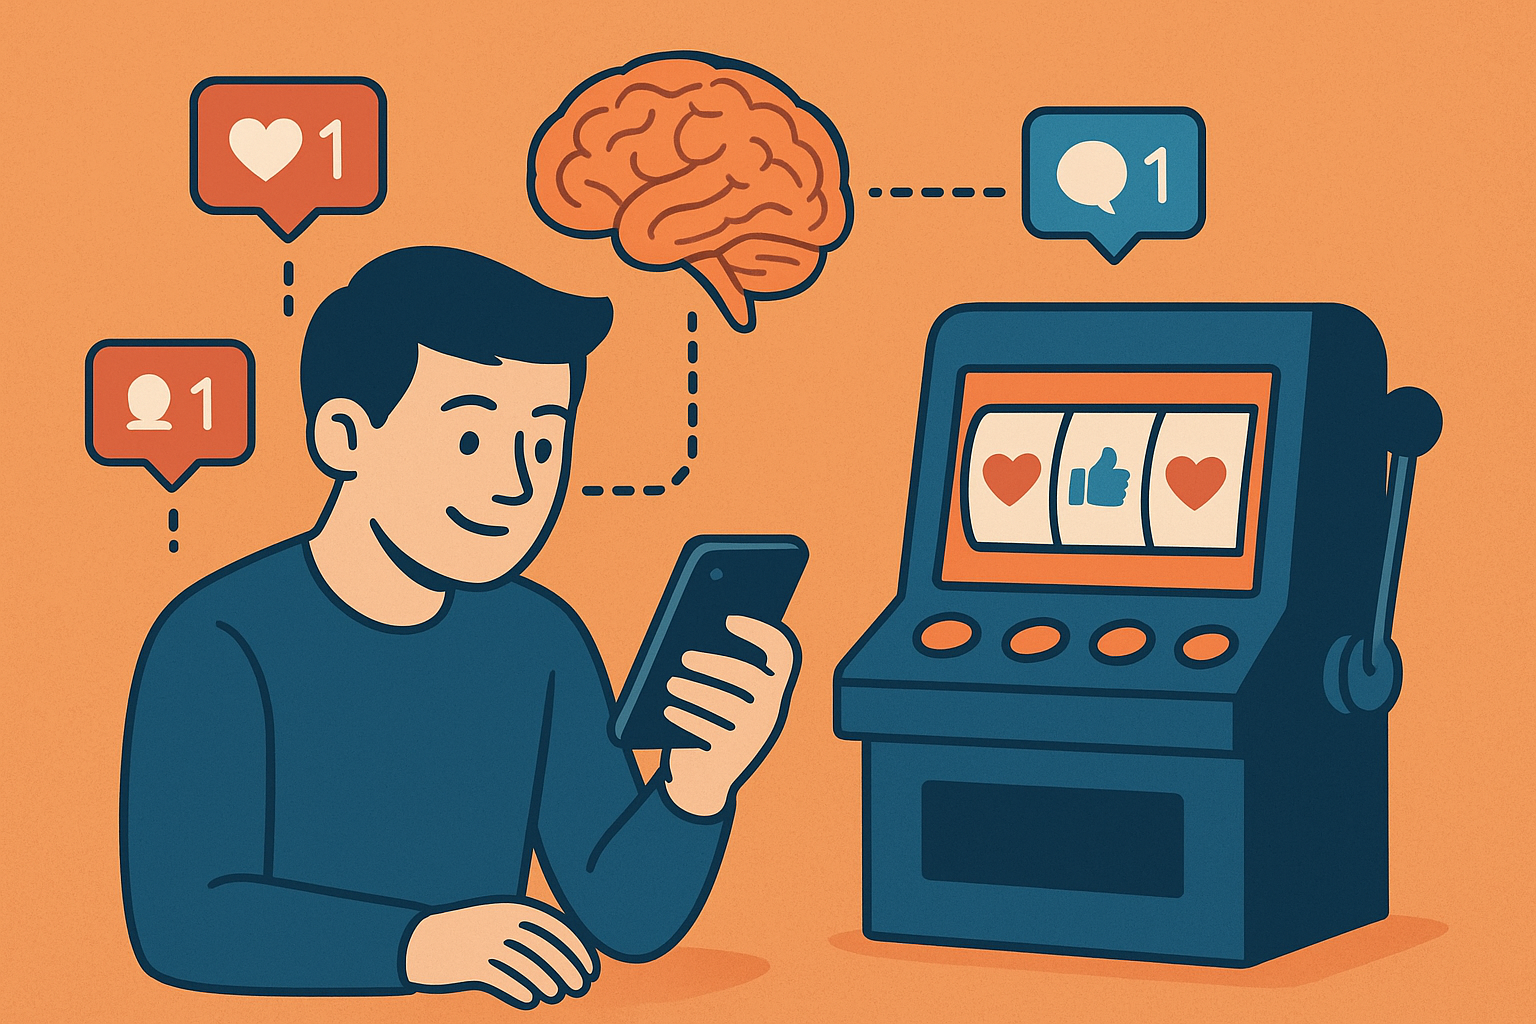
\includegraphics[width=\linewidth]{img/dopamina_1.png}
                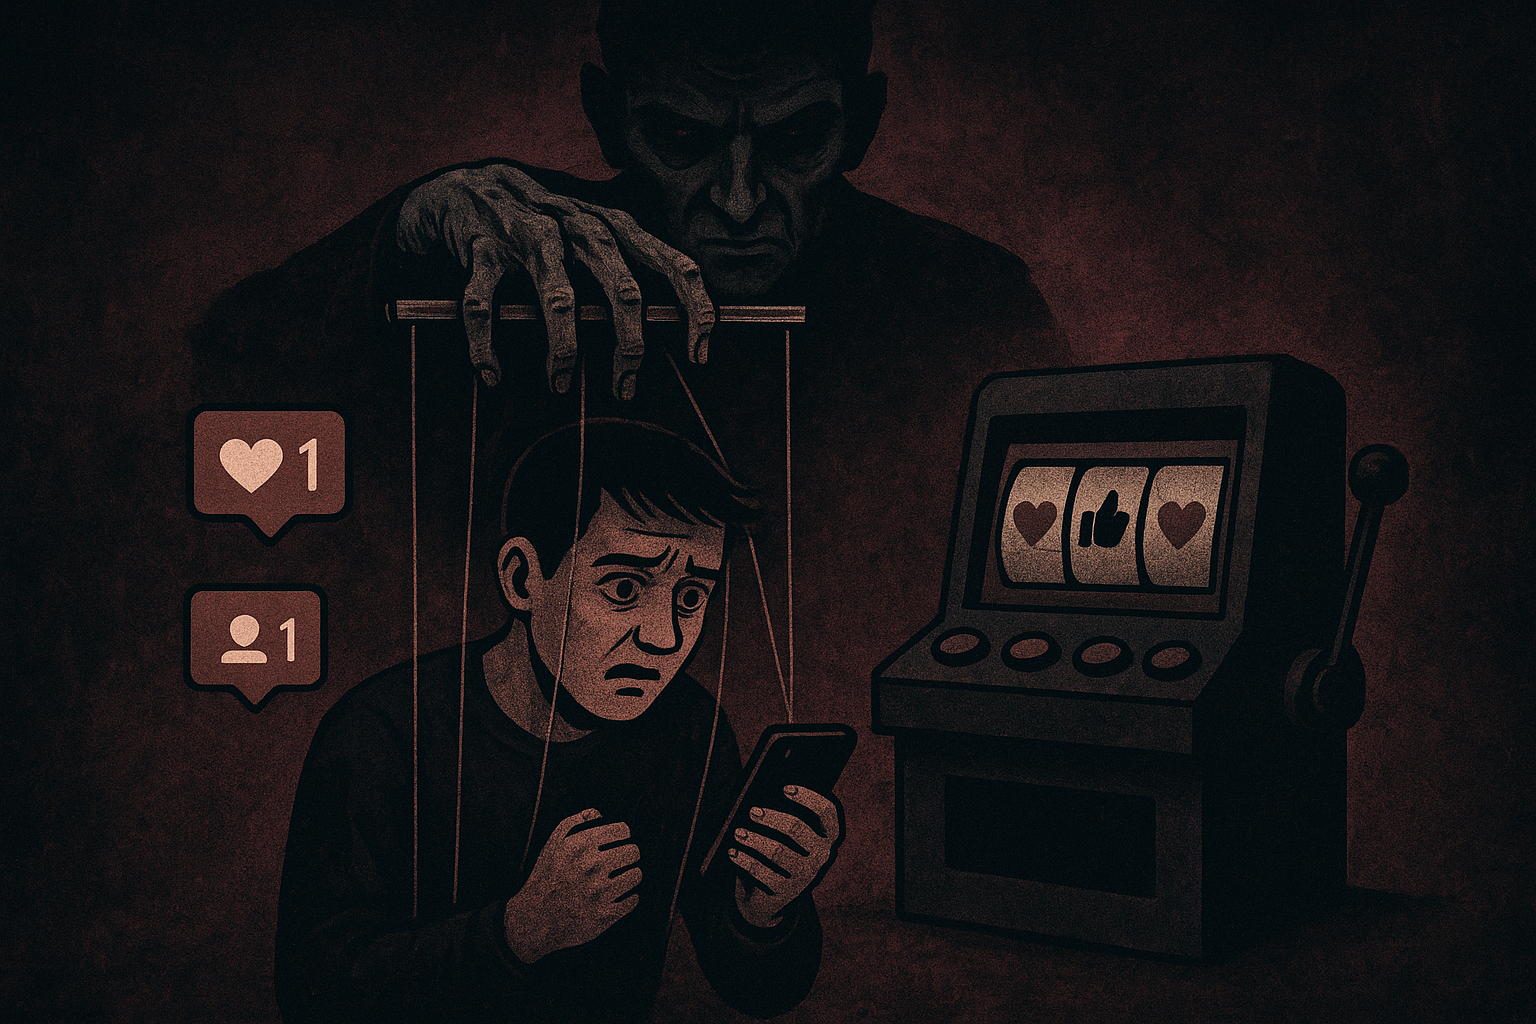
\includegraphics[width=\linewidth]{img/dopamina_2.png}
                \caption{{create con \href{https://chatgpt.com/}{ChatGPT}}}
            \end{figure}
    \end{columns}
\end{frame}

\begin{frame}{CATTURARE L'ATTENZIONE E CREARE DIPENDENZA}
    \begin{alertblock}{DARK PATTERN}
        \begin{minipage}{0.98\linewidth}
            \justifying
            I \textbf{dark pattern} sono interfacce progettate in modo da indurre gli utenti a compiere 
            azioni che altrimenti non compirebbero, come accettare termini di servizio sfavorevoli, 
            iscriversi a newsletter indesiderate o effettuare acquisti non intenzionati. 
            Questi design sfruttano principi psicologici per manipolare il comportamento 
            degli utenti, spesso a loro insaputa.\\
            \bigskip
            \tiny{\textbf{Esempio}}\\
            \tiny{\href{https://multiplayer.it/notizie/fortnite-epic-games-multa-da-520-milioni-per-aver-indotto-i-minori-ad-acquisti-indesiderati.html}{Fortnite: Epic Games multa da 520 milioni per aver indotto i minori ad acquisti indesiderati}}
        \end{minipage}
    \end{alertblock}
\end{frame}

\begin{frame}{CATTURARE L'ATTENZIONE E CREARE DIPENDENZA}
    \begin{minipage}{0.98\linewidth}
        \centering
        \Large
        \textit{``Io sono posseduto dall’altro; lo sguardo d’altri forma il mio corpo 
        nella sua nudità, lo fa nascere, lo scolpisce, lo produce, come è, 
        lo vede come io non lo vedrò mai. L’altro possiede un segreto: il segreto di ciò 
        che io sono. […] Così il senso profondo del mio essere è fuori di me, imprigionato 
        in un’assenza; altri è in vantaggio su di me.''}\\
        \bigskip
        \textbf{L'ENFER, C'EST LES AUTRES}
    \end{minipage}\\
    \bigskip
    \tiny{\textbf{Citazione}}\\
    \tiny{\href{https://arenaphilosophika.it/linferno-sono-gli-altri/}{J.P. Sartre, Porta chiusa}}
\end{frame}

\begin{frame}{QUALI DATI?! ESEMPIO: POLICY PRIVACY TIK TOK}
    \begin{figure}
        \href{https://www.tiktok.com/legal/page/eea/privacy-policy/it}{
\includegraphics[width=\linewidth]{img/tiktok_2.png}}
        \caption{{creata con \href{https://www.canva.com}{Canva}}}
    \end{figure}
\end{frame}

\section{ALTRE PROBLEMATICIT\'A DEI SOCIAL NETWORK}

\begin{frame}{DISINFORMAZIONE E CENSURA}
    \begin{figure}
        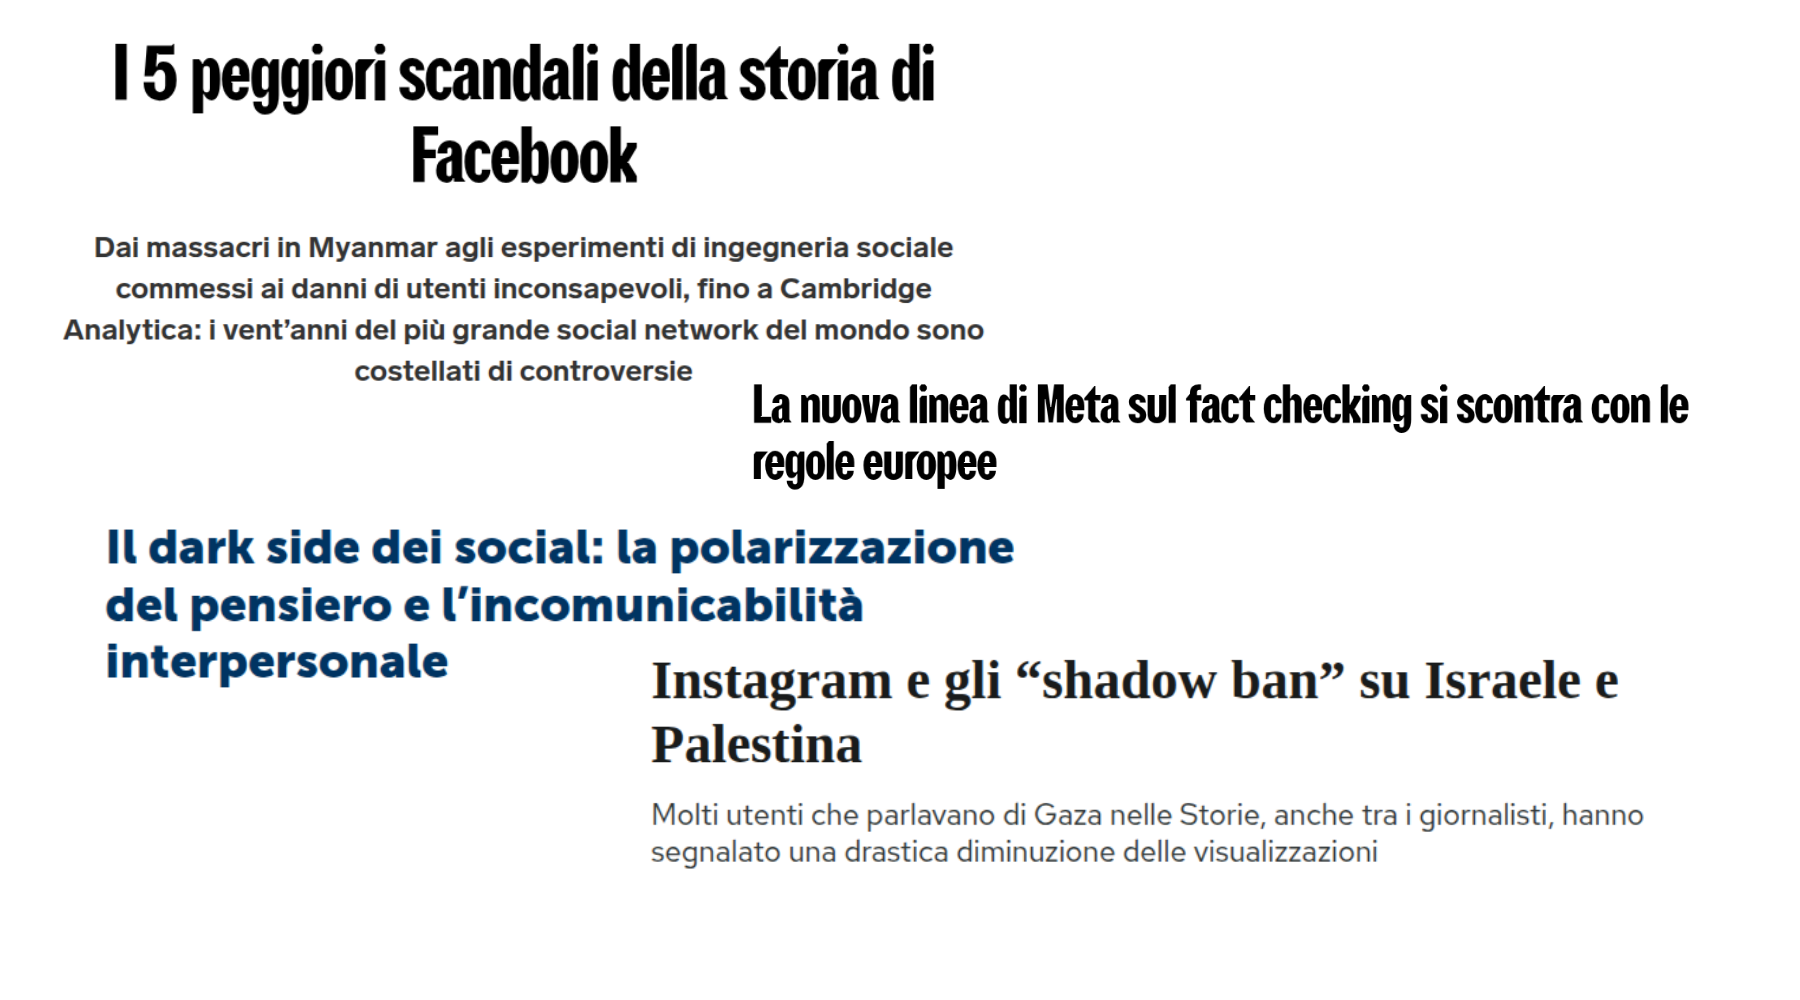
\includegraphics[width=.65\linewidth]{img/disinformazione.png}
        \caption{
            Immagine creata utilizzando screenshots tratti dai seguenti articoli:
            \href{https://www.ilpost.it/2023/10/19/shadow-ban-palestina-instagram/}{Il Post},
            \href{https://www.wired.it/article/meta-fact-checking-regole-europee-scorza/}{Wired: Marco Schiaffino},
            \href{https://www.wired.it/article/facebook-peggiori-scandali-cambridge-analytica-pubblicita-trump/}{Wired: Andrea Daniele Signorelli}
            \href{https://www.rizzolieducation.it/news/il-dark-side-dei-social-la-polarizzazione-del-pensiero-e-lincomunicabilita-interpersonale/}{Rizzoli Education}
        }
    \end{figure}
    \pause
    \begin{alertblock}{PROBLEMA DI GRANDEZZA DI SCALA}
        \begin{minipage}{0.96\linewidth}
            \justifying
            I social network e in generale le piattaforme online non affrontano in modo 
            adeguato il problema della \textbf{grandezza di scala} nella gestione dei contenuti 
            generati dagli utenti. Non esistono regole incrementali basate sull’audience.
        \end{minipage}
    \end{alertblock}
\end{frame}

\begin{frame}{CONSENSO AL TRATTAMENTO DEI DATI}
    \begin{alertblock}{PAY OR OK}
        \begin{minipage}{0.98\linewidth}
            \justifying
            Immagina di entrare in un sito web o un’app e trovarti di fronte a un 
            messaggio del tipo: ``\textbf{Accetta i cookie e la pubblicità personalizzata, 
            oppure paga un abbonamento per continuare}''. Questa è la logica del 
            modello ``Pay or OK'', conosciuto anche come ``Consent or Pay''. In pratica 
            l’utente viene messo davanti a una scelta crudele: \textbf{o cedere i propri dati 
            personali per la profilazione pubblicitaria, o pagare in denaro per preservare 
            la propria privacy}.\\
            \bigskip
            \tiny{\textbf{Fonte}}\\
            \tiny{\href{https://finto-consenso.hermescenter.org/problema/}{Finto consenso (Hermescenter)}}
        \end{minipage}
    \end{alertblock}
\end{frame}

\begin{frame}{EFFETTI DI SMARTPHONE E SOCIAL NETWORK}
    \begin{alertblock}{INFLUENZA SUL RENDIMENTO SCOLASTICO}
        \begin{minipage}{0.98\linewidth}
            \justifying
            L’indagine offre per la prima volta evidenze statistiche sugli \textbf{effetti dell’accesso 
            precoce ai dispositivi digitali sulle performance scolastiche}, utilizzando dati longitudinali 
            raccolti su 6.609 studenti di classi seconde e terze di scuole secondarie di secondo grado 
            in Lombardia. La ricerca ha analizzato il \textbf{legame tra l’età di primo utilizzo di smartphone 
            e social network e il rendimento scolastico}, unendo le risposte degli studenti a un questionario 
            con i loro risultati nei test INVALSI (Istituto Nazionale per la Valutazione del Sistema Educativo).\\
            Dai dati \textbf{emerge che gli studenti che aprono un profilo social in prima media ottengono punteggi 
            mediamente più bassi nelle prove standardizzate di italiano e matematica rispetto a 
            chi aspetta i 14 anni}, il limite fissato dalla normativa europea.\\
            \bigskip
            \tiny{\textbf{Rendimento scolastico dell'accesso precoce a smartphone e social}}\\
            \tiny{\href{https://www.unimib.it/news/presentata-milano-bicocca-ricerca-eyes-dedicata-agli-effetti-sul-rendimento-scolastico-dellaccesso}{Ricerca EYES UP}}
        \end{minipage}
    \end{alertblock}
\end{frame}

\begin{frame}{ENSHITTIFICATION}
    \begin{columns}
        \column{.75\textwidth}
            \begin{alertblock}{DEFINIZIONE}
                \begin{minipage}{0.96\linewidth}
                    \justifying
                    Il termine \textbf{enshittification} indica l’insieme di decisioni che porta 
                    una piattaforma di successo a diventare progressivamente meno piacevole e 
                    utilizzabile per i suoi utenti, fino a entrare in crisi. ``Ecco come muoiono 
                    le piattaforme'' scrisse Cory Doctorow: ``\textbf{prima trattano bene i loro utenti; poi ne 
                    abusano per favorire i loro clienti; infine, abusano dei loro stessi clienti 
                    per recuperare tutto il valore per sé stessi. E poi muoiono}''. 
                    Il processo è accelerato anche tramite contenuti \textbf{AI slop} ovvero 
                    contenuti digitali realizzati con l'intelligenza artificiale generativa, 
                    in particolare quando vengono percepiti come privi di impegno, qualità e 
                    significati profondi e caratterizzati da un volume di produzione eccessivo.\\
                    \bigskip
                    \tiny{\textbf{Fonte}}\\
                    \tiny{\href{https://www.ilpost.it/2023/08/03/enshittification/}{Il Post: le grandi piattaforme sono sempre peggio}}
                \end{minipage}
            \end{alertblock}
        \column{.25\textwidth}
            \begin{figure}
                
\includegraphics[width=.7\linewidth]{img/shit.png}
                \caption{{creata con \href{https://chatgpt.com}{ChatGPT}}}
            \end{figure}
    \end{columns}
\end{frame}

\begin{frame}{SOCIAL NETWORK ETICO}
    \begin{columns}
        \column{.6\textwidth}
            \justifying
            \textbf{Social networking che non è in vendita}.\\
            La tua home feed dovrebbe essere riempita con ciò che conta di più per te, 
            non con ciò che una corporazione pensa che dovresti vedere. Social media 
            radicalmente diverso, di nuovo nelle mani delle persone.\\
            \bigskip
            \tiny{\textbf{MASTODON}}\\
            \tiny{\href{https://joinmastodon.org/it}{Cos'è e come funziona Mastodon?}}\\
            \bigskip
            \tiny{\textbf{SOCIALINI}}\\
            \tiny{\href{https://socialini.it/}{Socialini: esperimento pedagogico}}
        \column{.4\textwidth}
            \begin{figure}
                
\includegraphics[width=\linewidth]{img/mastodon.png}
                \caption{{Fonte: \href{https://joinmastodon.org/it}{Mastodon}}}
            \end{figure}
    \end{columns}
\end{frame}

\end{document}